\section{Summary}
\label{chap:correctness:summary}

\mnote{Insight}
In this chapter, we have discussed notions of correctness for transformation networks and the artifacts they consist of, and we have precisely defined the notion that is relevant for the context of this thesis.
We give an overview of the introduced concepts and their relations in the conceptual model in \autoref{fig:correctness:conceptual_model}.
In summary, we provided the following insight in this chapter.

\begin{insight}[Correctness Notion]
    A reasonable notion of correctness for networks of modular, independently developed transformations consists of correctness of the single transformations, which need to be synchronizing, and correctness of the application function that determines an execution order of the transformations.
    An application function may not be able to return a result due to different reasons, such as transformations not being applicable to specific changes, the absence of an execution order of the transformations that leads to consistent models, or the inability to find such an order.
    Thus, in comparison to correctness, the degree of conservativeness is the more important property of an application function, which indicates how often the function does not deliver a result although there is an order of transformations that would restore consistency.
    Additionally, although theoretically not relevant for correctness, the relations defining when models are considered consistent have to fulfill some notion of compatibility to be useful, as they can otherwise prevent transformations from finding consistent models.
    %Finally, we found that we can define a more fine-grained notion of consistency that is aligned with practical representations of consistency in transformation languages.
\end{insight}

\mnote{Achieving correct transformation networks}
In the following chapters, we will thus define a notion of compatibility for consistency relations, discuss how correctness of the individual synchronizing transformations for achieving local consistency can be achieved, and finally how a correct and appropriate application function to perform the orchestration for achieving global consistency can be defined.
In summary, these following contributions together will allow to develop what we defined as a \emph{correct} transformation network.

\begin{figure}
    \centering
    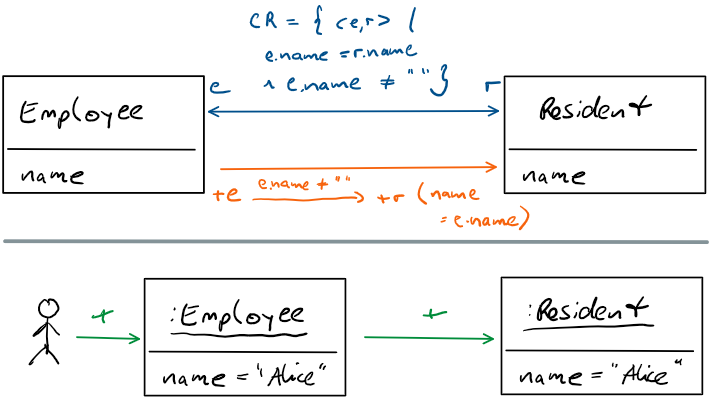
\includegraphics[width=0.8\textwidth]{figures/correctness/notion/visualization_example.png}
    \caption[Example for concept visualizations]{Example for visualization of consistency relations, consistency preservation rules and their execution.}
    \label{fig:correctness:visualization_example}
\end{figure}

For visualizing examples of consistency relations, consistency preservation rules and their execution throughout the next chapters, we use a notation according to the example depicted in \autoref{fig:correctness:visualization_example}.
We visualize consistency relations in blue with a definition of the conditions for consistency relation pairs forming that relation.
In the example, the consistency relation contains all pairs of employees and residents having the same name, expect for those with an empty name.
We depict consistency preservation rules in orange and denote which changes it produces because of which input change.
In the example, we denote that the addition of an employee ($+e$) leads to the addition of a resident with the same name, specified by the according property assignment $r(\mathvariable{name} = \mathvariable{e.name})$.
In addition, we annotate conditions to the consistency preservation rules, such as $\mathvariable{e.name} \neq \textnormal{\enquote{}}$ in the example, which restricts the resident creation to the case in which the employee has a non-empty name.
We usually specify only parts of a consistency preservation rule, e.g., in the example we only specify the behavior for the case of adding an element but not of modifying or removing it.
Finally, we denote the execution of any changes, including consistency preservation rules, in green.
In the example, we visualize the addition of an employee by a user, denoted with a $+$, which leads to the addition of a resident, for example, because of the execution of the above introduced consistency preservation rule.


% \section{Summary}

% Central Insights:
% \begin{itemize}
%     \item In networks, we need compatible consistency relations -> first RQ
%     \item In networks, we need synchronizing rather than bidirectional transformations -> second RQ
%     \item In networks, we need orchestration functions -> third RQ
%     \item Correctness is not the problem, optimality is the problem
%     \item We can only check dynamically whether a consistent state was reached due to Halting Problem. We cannot guarantee to always find a consistent state
% \end{itemize}